%%%%%%%%%%%%%%%%%%%%%%%%%%%%%%%%%%%%%%%%%%%%%%%%%%%%%%%%%%%%%%%%%%%%%%%%%%%%%%
%
% タイトル TeX用テンプレート 
% バージョン 2014-11-8 (Sat) 初版
% 作成者 Kouhei Ito
% 作成場所 野々市市中林 DeuxMKK
% 用途 2段組レポートの作成等
%
%%%%%%%%%%%%%%%%%%%%%%%%%%%%%%%%%%%%%%%%%%%%%%%%%%%%%%%%%%%%%%%%%%%%%%%%%%%%%%%%
%\documentclass[11pt,twocolumn]{jsarticle}
\documentclass[11pt]{jsarticle}
\usepackage[dvipdfmx]{graphicx}
\usepackage{amsmath,amssymb}
\usepackage{url}
\usepackage{nidanfloat}

%% 体裁

% ページレイアウト(A4:297 mm × 210 mm,1 インチ = 25.4 mm)
% http://www.biwako.shiga-u.ac.jp/sensei/kumazawa/tex/layout.html
% http://www.slis.tsukuba.ac.jp/~fujisawa.makoto.fu/cgi-bin/wiki/index.php?TeX%A5%E1%A5%E2#p61e1b46
% 上 20 mm,下 22 mm,左右 20 mm の余白設定
\setlength{\topmargin}{-20truemm}
\setlength{\headheight}{10truemm}
\setlength{\headsep}{4.6truemm}
\setlength{\textheight}{255truemm}
\setlength{\oddsidemargin}{-5.4truemm}
\setlength{\evensidemargin}{-5.4truemm}  % twoside オプション指定時のみ有効
\setlength{\textwidth}{170truemm}
% \setlength{\columnsep}{8truemm}
\setlength{\columnsep}{6truemm}


%%%%%%%%%%%%%%%%%%%%%%%%%%%%%%%%%%%%%%%%%%%%%%%%%%%%%%%%%%%%%%%%%%%%%%%%%%%%%%%%
\title{音声認識による接客ロボットの開発}
\author{金沢工業高等専門学校 澤田茂人}
\date{2016-8-23}
%%%%%%%%%%%%%%%%%%%%%%%%%%%%%%%%%%%%%%%%%%%%%%%%%%%%%%%%%%%%%%%%%%%%%%%%%%%%%%%%
\begin{document}
\maketitle
\begin{abstract}
音声認識について今から解説する。音声認識とは、人間の声などをコンピューターに認識させることであり、話し言葉を文字列に変換したり、あるいは音声の特徴をとらえて声を出している人を識別する機能を指す。

\end{abstract}

\tableofcontents
%%%%%%%%%%%%%%%%%%%%%%%%%%%%%%%%%%%%%%%%%%%%%%%%%%%%%%%%%%%%%%%%%%%%%%%%%%%%%%%%
\section{はじめに}
今回の音声認識は食堂にて注文を取るロボットがある場合、人件費等の経費削減ができるため制作してほしいという要望があった。食堂で注文を取るロボに使用した音声を認識させるシステムについて述べていく。

\subsection{研究の背景}
食堂にて注文を取るロボットがある場合、人件費等の経費削減ができるため制作してほしいという要望があり音声でのやりとりをするためのシステムを究明する必要があると考える。

\subsection{研究の目的}
linuxPCに音声認識をするためjulius、Open-JTalkを用意して人間の声をマイクから拾い、実際に店で使用することを目的とする。図1に音声認識をしようとした時のイメージを示す。


\begin{figure*}[b]
 \begin{center}
  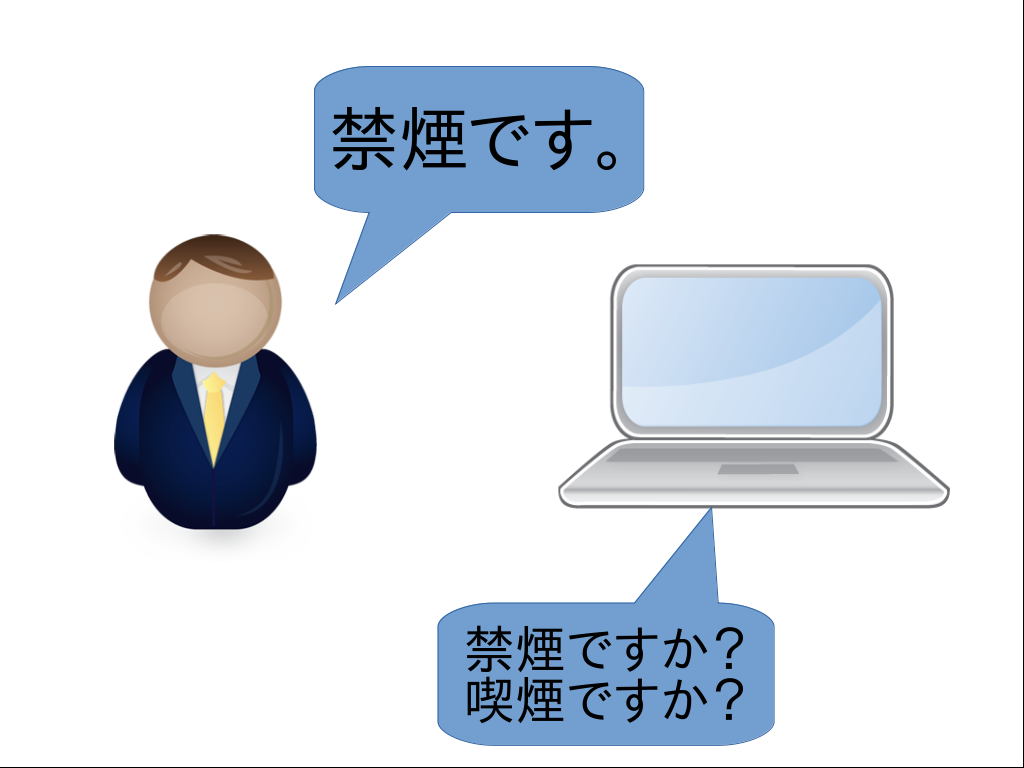
\includegraphics[width=90mm]{sukusho.png}
  \caption{様子}
  \label{fig:kinshi}
 \end{center}
\end{figure*}

\subsubsection{julius,Open-JTalk}
Julius は,音声認識システムの開発・研究のためのオープンソースの高性能な汎用大語彙連続音声認識エンジンである。数万語彙の連続音声認識を一般のPC上でほぼ実時間で実行できる。また,高い汎用性を持ち,発音辞書や言語モデル・音響モデルなどの音声認識の各モジュールを組み替えることで,様々な幅広い用途に応用できる。[1]ここではオリジナルの言語モデルを使用したため、図2、図3、図4、図5、図6、図7、図8に示す。Open-JTalkは、日本語テキストを音声に変換するシステムである。[2]

\begin{figure*}[b]
 \begin{center}
  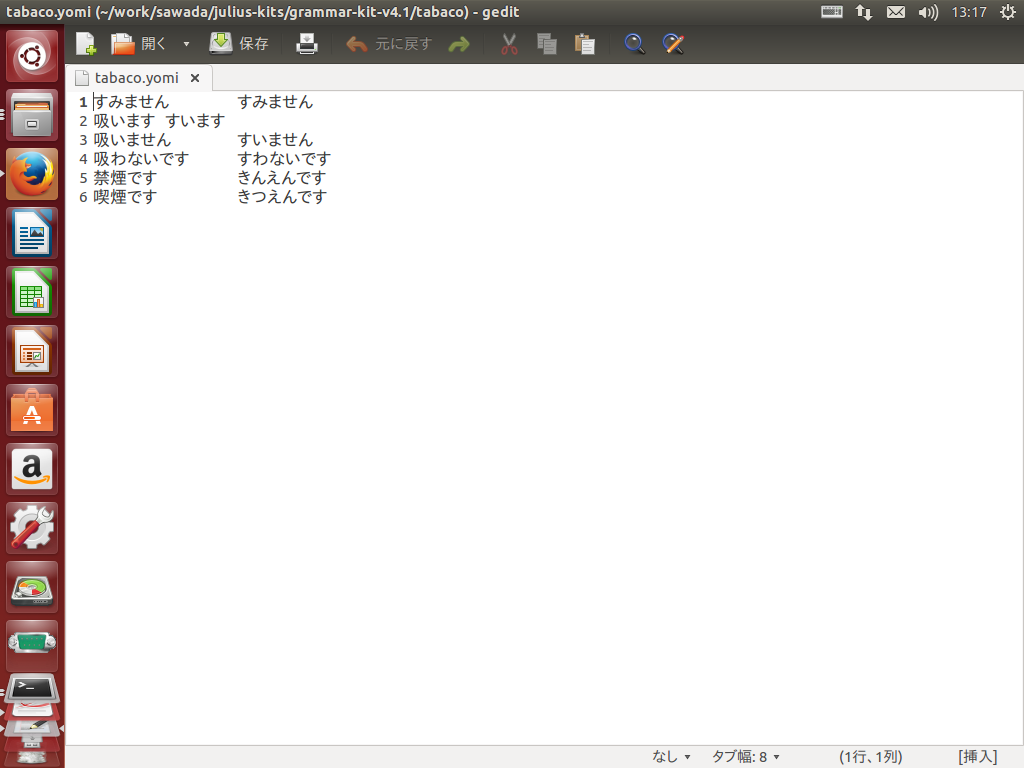
\includegraphics[width=90mm]{yomi.png}
  \caption{yomiファイル}
  \label{fig:kinshi}
 \end{center}
\end{figure*}

\begin{figure*}[b]
 \begin{center}
  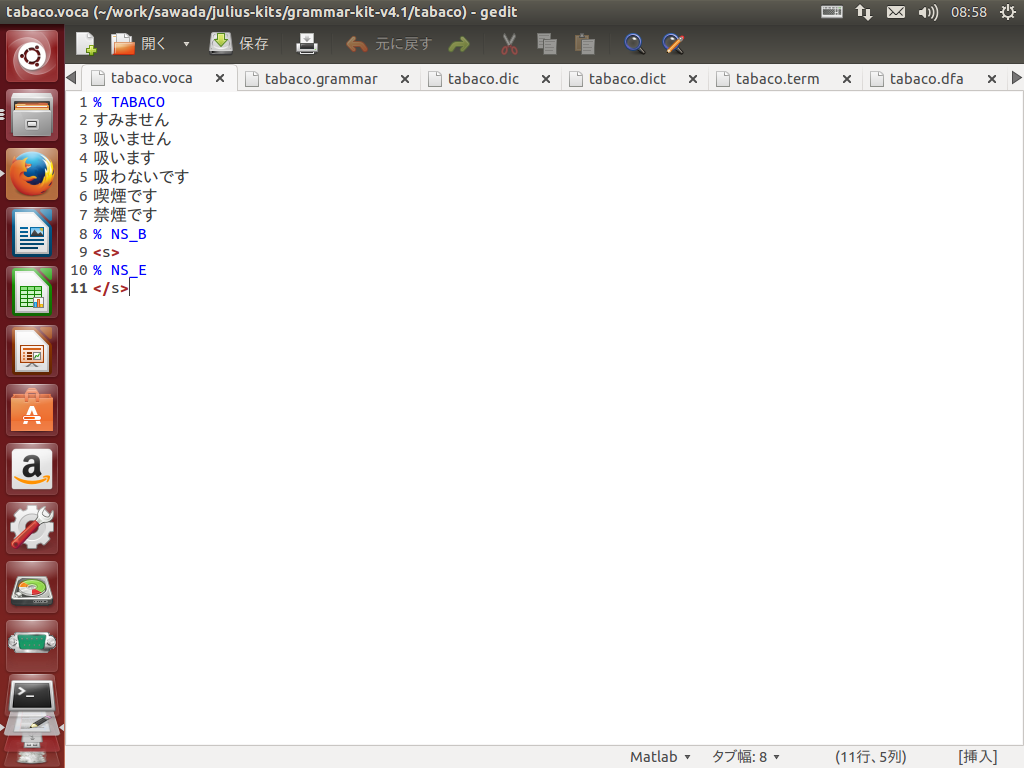
\includegraphics[width=90mm]{voca.png}
  \caption{vocaファイル}
  \label{fig:kinshi}
 \end{center}
\end{figure*}

\begin{figure*}[b]
 \begin{center}
  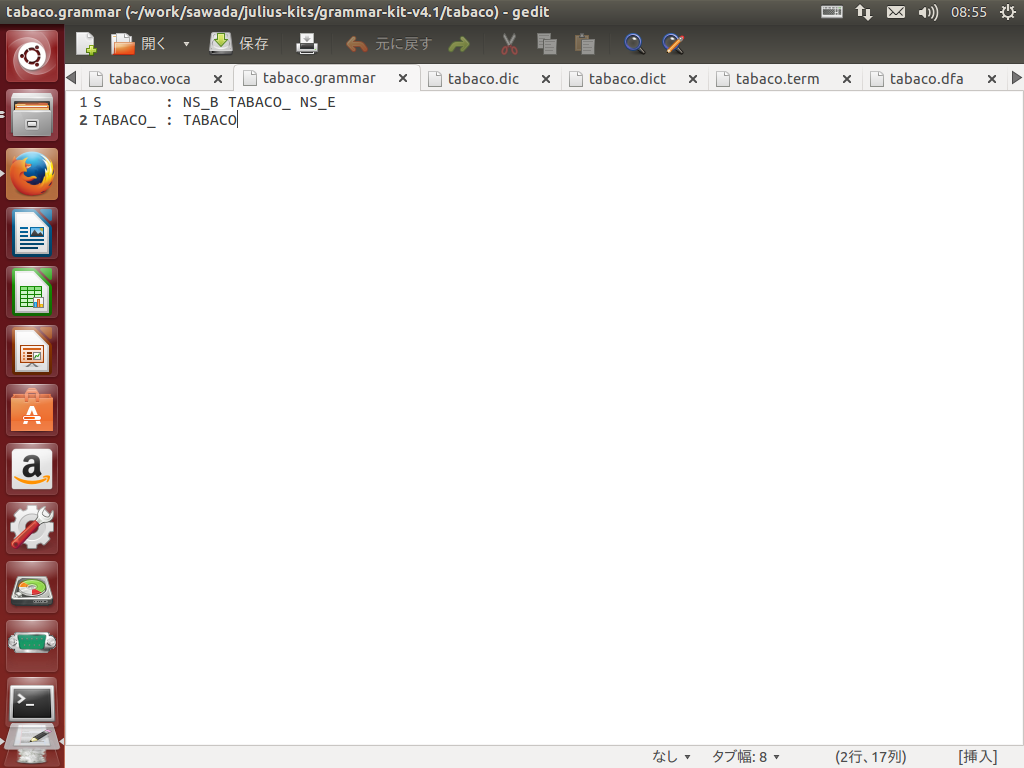
\includegraphics[width=90mm]{grammar.png}
  \caption{grammarファイル}
  \label{fig:kinshi}
 \end{center}
\end{figure*}

\begin{figure*}[b]
 \begin{center}
  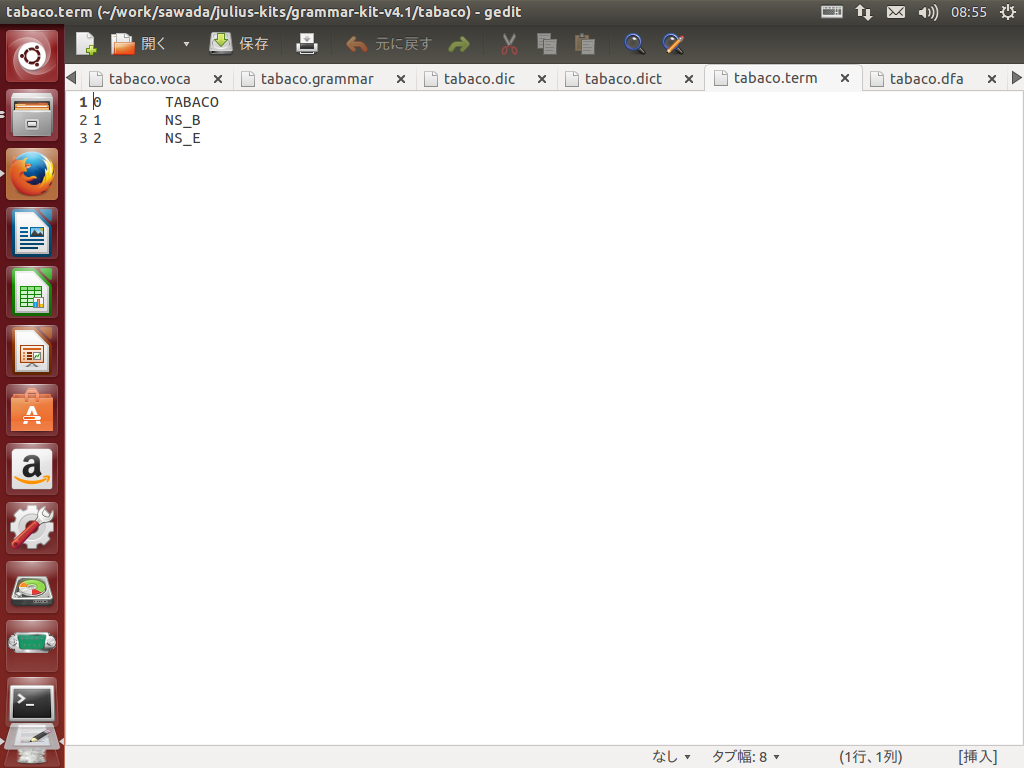
\includegraphics[width=90mm]{term.png}
  \caption{termファイル}
  \label{fig:kinshi}
 \end{center}
\end{figure*}

\begin{figure*}[b]
 \begin{center}
  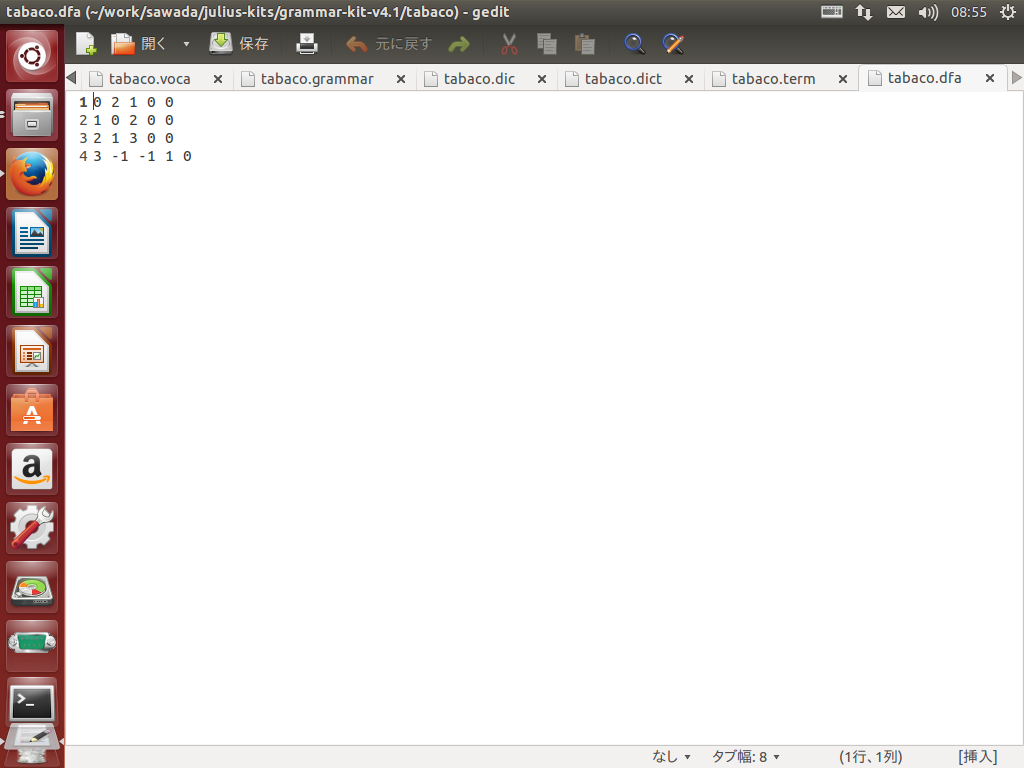
\includegraphics[width=90mm]{dfa.png}
  \caption{dfaファイル}
  \label{fig:kinshi}
 \end{center}
\end{figure*}

\begin{figure*}[b]
 \begin{center}
  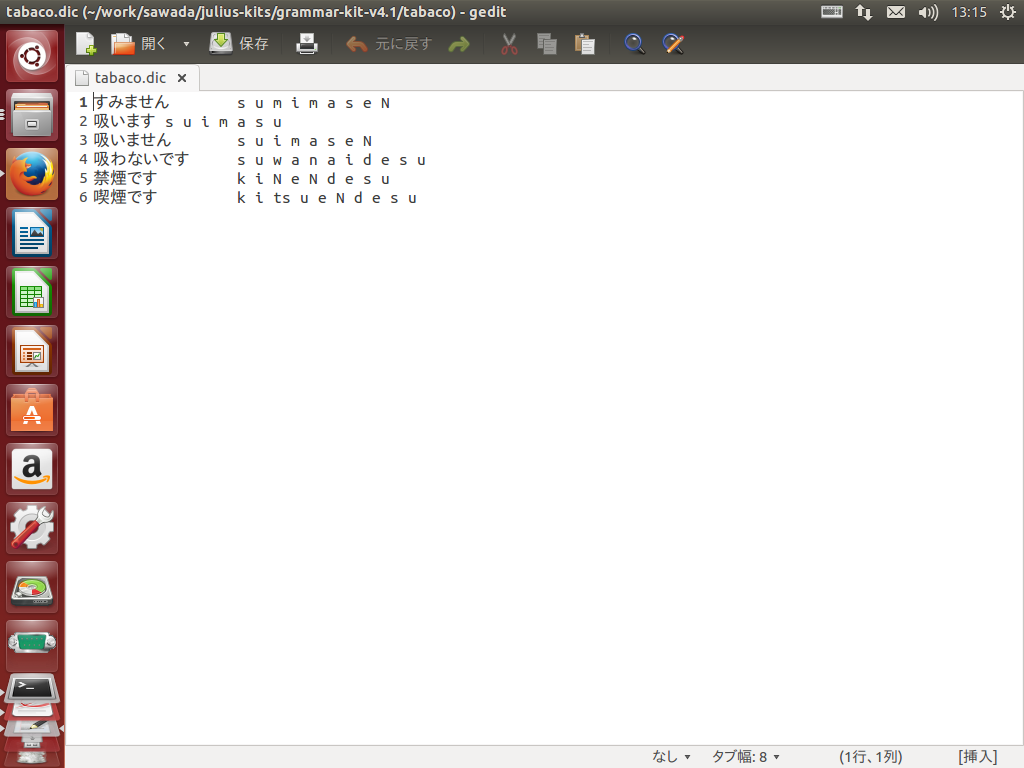
\includegraphics[width=90mm]{dic.png}
  \caption{dicファイル}
  \label{fig:kinshi}
 \end{center}
\end{figure*}

\begin{figure*}[b]
 \begin{center}
  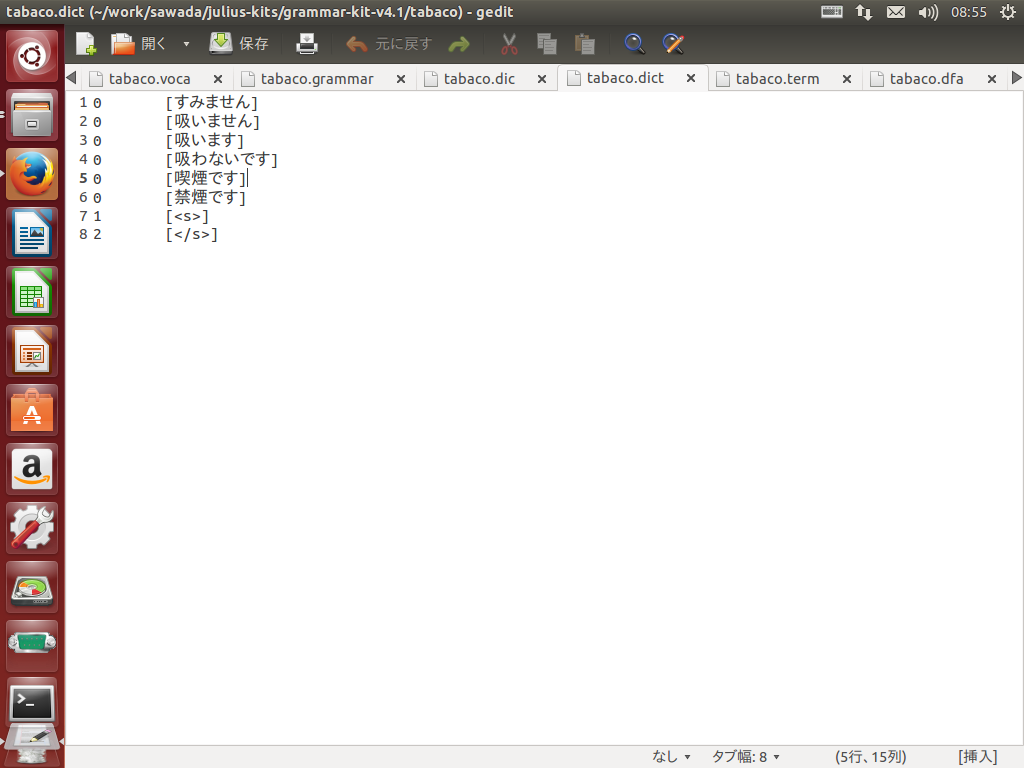
\includegraphics[width=90mm]{dict.png}
  \caption{dictファイル}
  \label{fig:kinshi}
 \end{center}
\end{figure*}

\section{研究手順}
【julius】


https://github.com/julius-speech/juliusよりjulius 4.3.1をcloneする。


https://osdn.jp/projects/julius/downloads/60416/dictation-kit-v4.3.1-linux.tgz/ よりディクテーションキットをダウンロードし、解凍する。


https://osdn.jp/projects/julius/downloads/51159/grammar-kit-v4.1.tar.gz/ よりディクテーションキットをダウンロードし、解凍する。


cd julius-4.3.1/


./configure


make


sudo make instal


テキストファイルにてgrammarファイルとyomiファイル図2、図3に習って書く。


yomi2voca.pl tabaco.yomi > tabaco.vocaと打ち込むと図4が出力される。


mkdfa.pl tabacoと打ち込むと図5、図6、図7、図8が出力される。


generate tabacoと打つことで文法から文をランダム生成することができる。[3]その様子を図9に示す。

\begin{figure*}[b]
 \begin{center}
  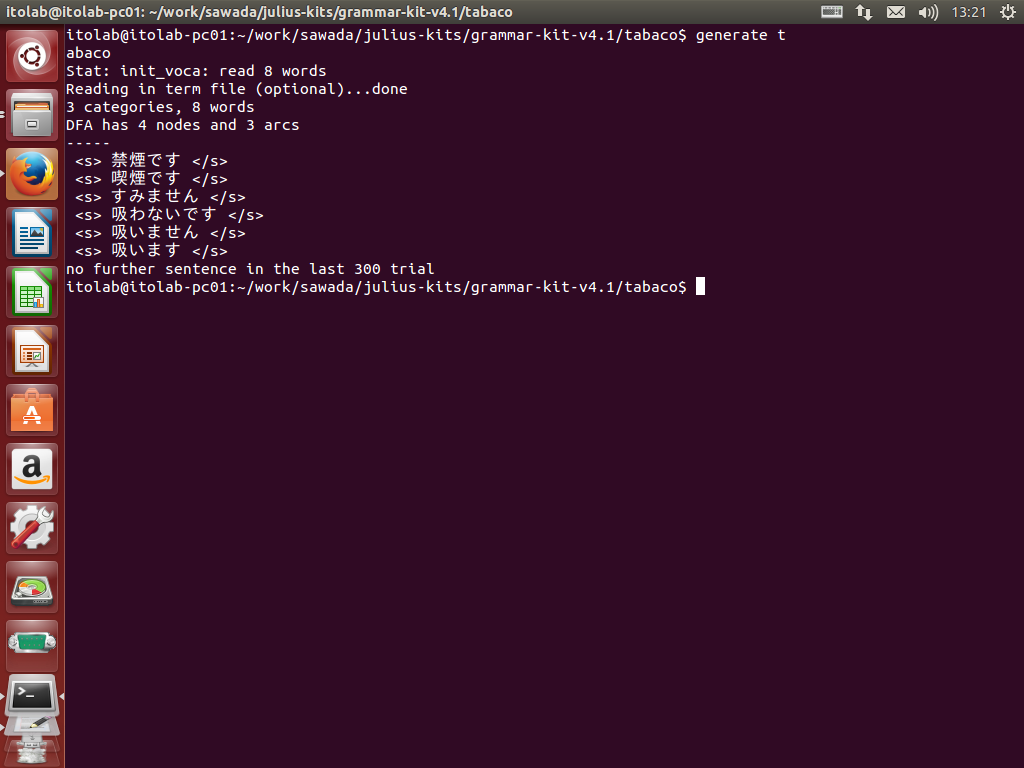
\includegraphics[width=90mm]{generate.png}
  \caption{generate}
  \label{fig:kinshi}
 \end{center}
\end{figure*}


tabaco.jconfとtabaco.dicをgrammar-kit-v4.1に移動させる。


dictation-kit中でjulius -C tabaco.jconf -input mic -charconv EUC-JP UTF-8


と打ち込むことで音声を入力できる。


【Open-JTalk】


cppでプログラムを作成し、コンパイルする。今回はvoiceという名前で保存した。プログラムの中を図10に示す。

\begin{figure*}[b]
 \begin{center}
  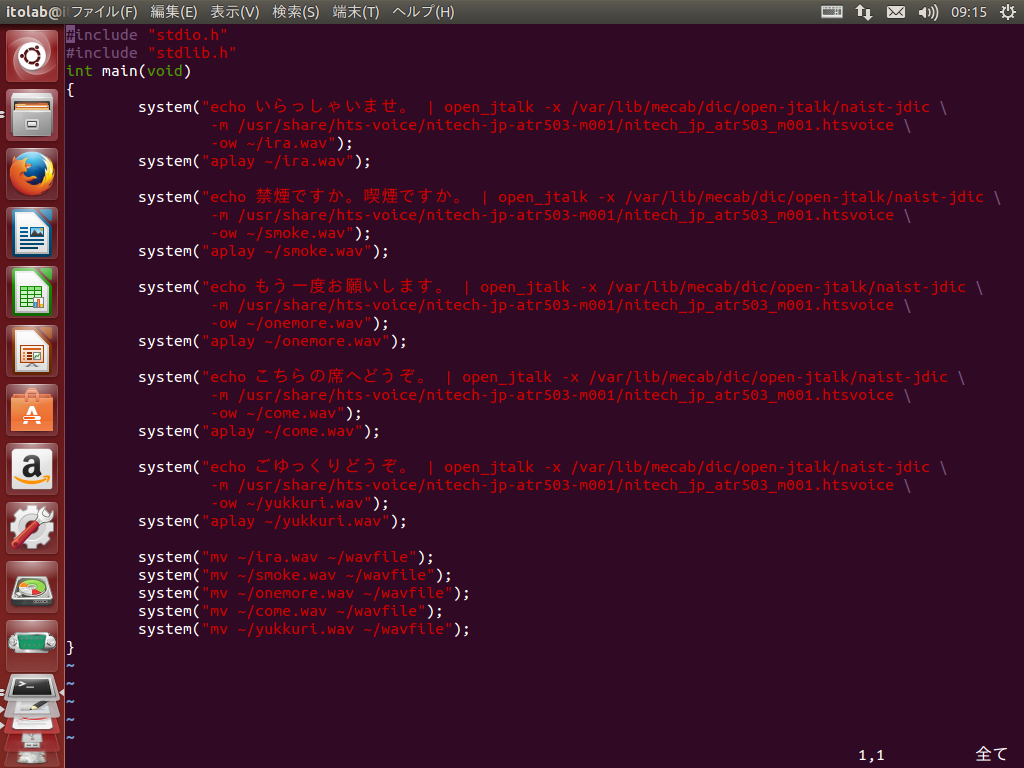
\includegraphics[width=90mm]{voice.png}
  \caption{プログラム}
  \label{fig:kinshi}
 \end{center}
\end{figure*}


\section{研究手順説明}
juliusは研究手順に示したコマンドを上から順にviにて打ち込む。Open-JTalkは図8に示したプログラムを組み、コンパイルさせることで音声を出力させることができる。


\section{研究結果}
juliusで音声を入力し、認識することを確認した。そのときの様子を図11に示す。Open-Jtalkでは自作のプログラムを組み、必要な音声を出力することに成功した。そのときの様子を図12に示す。

\begin{figure*}[b]
 \begin{center}
  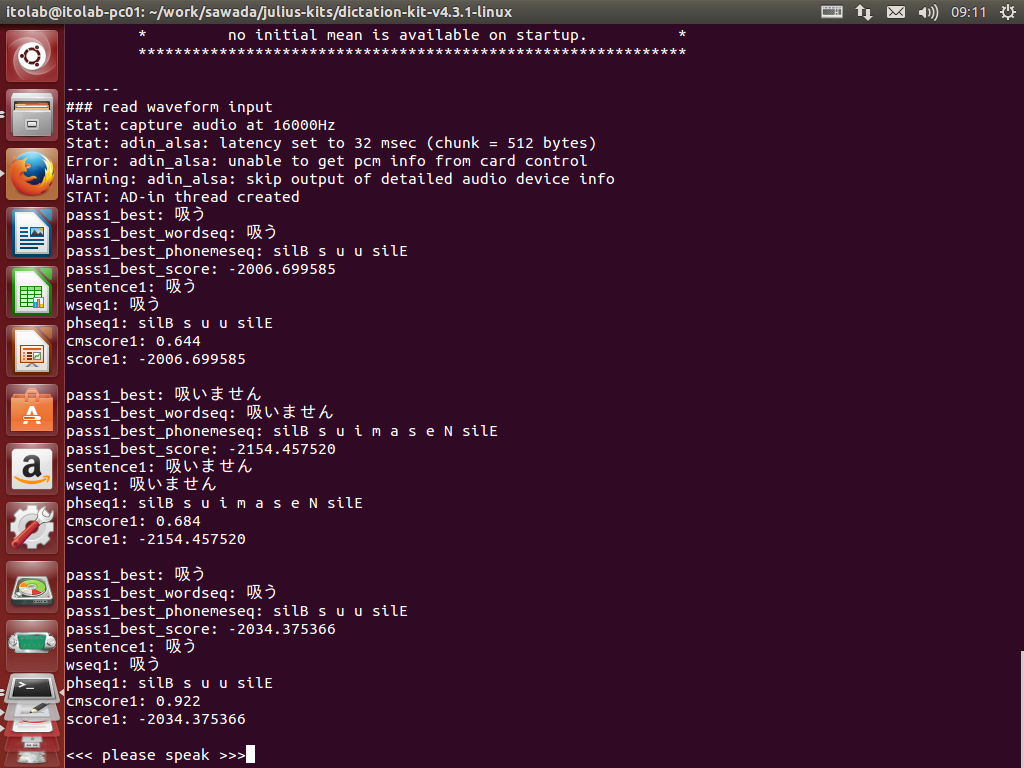
\includegraphics[width=90mm]{ninshiki.png}
  \caption{認識結果}
  \label{fig:kinshi}
 \end{center}
\end{figure*}

\begin{figure*}[b]
 \begin{center}
  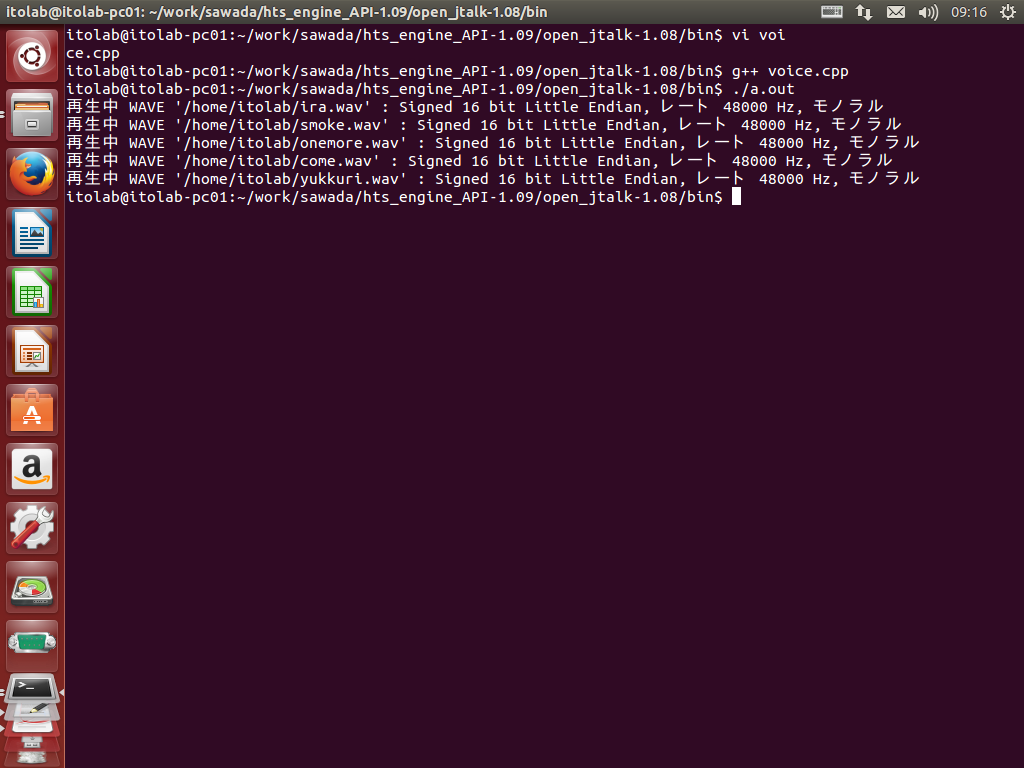
\includegraphics[width=90mm]{konpairu.png}
  \caption{音声の出力}
  \label{fig:kinshi}
 \end{center}
\end{figure*}

\section{考察}
今回はjuliusを使用して音声の入力やOpen-JTalkを使用して音声の出力を行うことができたがそれぞれ独立して操作を行ったため、juliusを使用する際にテキストファイルを出力させ、そのテキストファイルをOpen-JTalkが音声として出力させるためのツールを見つけて使用することができればこの研究は完成すると考えられる。


\section{おわりに}
今回ロボットに音声認識をさせることで人件費の削減につなげられるのではないかと考え、juliusやOpen-JTalkで音声の入出力を行うことと決めjuliusでの音声の認識やOpen-JTalkでの音声の出力に成功した。今後はjuliusとOpen-JTalkを連携する手段を見つけ、人間とロボットの対話を行えるようにする。

\section{参考文献}
[1] julius book http://julius.osdn.jp/juliusbook/ja/pr01.html


[2] Open JTalk - HMM-based Text-to-Speech System http://open-jtalk.sourceforge.net/


[3]generate https://julius.osdn.jp/juliusbook/ja/generate.html
%%%%%%%%%%%%%%%%%%%%%%%%%%%%%%%%%%%%%%%%%%%%%%%%%%%%%%%%%%%%%%%%%%%%%%%%%%%%%%%%%


\end{document}
